\documentclass[a4paper, 12pt]{article}
\usepackage[utf8]{inputenc}
\usepackage[T1]{fontenc}
\usepackage[english]{babel}
\usepackage{amsmath}
\usepackage{amssymb}
\usepackage{amsfonts}
\usepackage{mathtools}
\usepackage{graphicx}
\usepackage{caption}
\usepackage{subcaption}
\usepackage{float}
\usepackage{wrapfig}
\usepackage{array}
\usepackage{booktabs}
\usepackage{multirow}
\usepackage{colortbl}
\usepackage{xcolor}
\definecolor{darkgreen}{rgb}{0.0, 0.5, 0.0}
\usepackage{geometry}
\usepackage{fancyhdr}
\usepackage[backend=biber,style=apa,sorting=nyt]{biblatex}
\addbibresource{master.bib}
\geometry{left=1in, right=1in, top=1in, bottom=1in}
\setlength{\headheight}{14.49998pt}
\addtolength{\topmargin}{-2.49998pt}
\usepackage{setspace}
\onehalfspacing
\usepackage{hyperref}
\usepackage{bookmark}
\hypersetup{
    colorlinks=true,
    linkcolor=black,
    citecolor=black,
    urlcolor=black
}
\usepackage{listings}
\usepackage{algorithm}
\usepackage{algpseudocode}
\newcommand{\E}{\mathbb{E}}
\newcommand{\Var}{\mathrm{Var}}
\usepackage{siunitx}
\usepackage{csquotes}
\usepackage{enumitem}
\usepackage{lipsum}

\setlength{\parindent}{1.25cm}
\setlength{\parskip}{0.25cm}

\begin{document}
\pagestyle{fancy}
\fancyhf{}
\lhead{Lucas Dubois}
\rhead{\today}
\cfoot{\thepage}
\renewcommand{\headrulewidth}{0pt}
\begin{titlepage}
\vspace{12cm}
\par
\textit{Master Thesis in Economics with finality Macroeconomics and Finance}
\par
\textit{HEC Liege}
\par
\textit{Supervisor: Malka Guillot}
\par
2024-2025
\begin{center}
\rule{\linewidth}{1pt}
\vspace{0,5cm}
\vspace{0.75cm}
\begin{spacing}{1.75}
{\LARGE \textbf{\textit{Top-Income Inequality in Brazil: The Role of Dividend Taxation}}}
\vspace{0.75cm}
\end{spacing}
\rule{\linewidth}{1pt}
\vspace{0,5cm}
\\
\textbf{{\large Lucas Dubois}}
\\
\vspace{0,5cm}
{(s216283)}\end{center}
\vspace{0.5cm}
\begin{abstract}
    \hspace{1cm} As seen in the course, the New Keynesian (NK) model serves as a fundamental framework in macroeconomic theory and the formulation of monetary policy. 
At its core lies the concept of \textit{divine coincidence}, which suggests that stabilizing inflation successfully stabilizes the output gap that influences welfare. 
This finding significantly eases the challenges faced by central banks since it clearly implies that prioritizing inflation control is enough to reach market efficiency.
However, in their 2007 paper, Blanchard and Galí question this assumption by integrating the notion of \textit{real wage rigidities } in the NK framework. 
Their findings reveal that once we take these frictions into account, the divine coincidence disappears.
\end{abstract}

\vspace{3cm}

\begin{center}
{\Large \today}
\end{center}
\end{titlepage}
\tableofcontents
\newpage

In 1995, Brazil eliminated its dividend taxes, arguing that double taxation of corporate profits hindered growth and distorted capital allocation.
This tax policy, however, helped the consolidation of a very regressive tax system, in which the 85th percentile pays a higher average tax rate than the 99th by 2022 (Figure~\ref{tab:Figure 1}). 
Since then, inequality in Brazil has remained on the rise, confining the 7th most populous nation to a capital concentrating status quo. 
As of 2022, Brazil's Gini index is 53\%, making it the most unequal country in Latin America and among the top 10 globally\footnote{World Bank, 2022}.
Brazil also has the highest wealth concentration worldwide: the top 1\% holds 48.4\% of national wealth\footnote{Global Wealth Report, 2023}.
\par
Several recent studies have attempted to understand the role of taxation on top income inequality. 
Particularly, \cite{berman2024capital} investigate the impact of dividend taxes on top income inequality in Israel, following the 2017 tax cut. 
They find a significant increase in retained earnings among the top 1\%, which is not observed in other income groups.
Similarly, \cite{nallareddy2021corporate} study the effects of corporate taxes on income inequality, finding that corporate tax cuts led to increases in income inequality, a result that is robust across regressions.
Together, those studies provide a strong empirical framework that will serve as the foundation for my research.
\par
Considering the context of Brazil and the existing literature, I would like to dedicate my master’s thesis to understanding the drivers of top-income inequality in Brazil, with a particular focus on the role of dividend taxation in shaping income distribution.
The database provided by \href{https://wid.world/country/brazil/}{WID} offers a wealth of time series indicators related to income distribution and inequality, which will be crucial for my analysis.
In particular, the study by \cite{morgan2025distribution} presents an extensive analysis of the evolution of income, minimum wages, and wealth in Brazil over a 72-year period (\textit{see} Figure~\ref{tab:Figure 2}), by combining data from various official Brazilian agencies and other non-official microdata sources.
Moreover, the authors provide a well-structured use of the raw data they compiled, along with a solid theoretical framework to understand the evolution of income and wealth in Brazil.
\par    
My approach will be the Synthetic Control Method (SCM), which allows for the construction of a synthetic control group that approximates the characteristics of the treated unit.
This method is particularly useful when the number of treated units is small, as is the case for Brazil.
The SCM was formalized in \cite{abadie2003economic} and further developed in \cite{abadie2010synthetic}.
To improve the model’s efficiency, I will include a set of controls that capture the main determinants of income inequality, such as financial development, openness, government spending, and poverty rates, following the work by \cite{afandi2017determinants} and \cite{roine2009long}.
\pagebreak
\par
Furthermore, in order to optimize the model’s performance, I will use Machine Learning techniques to construct the synthetic controls, as described by \cite{araujo2023synthetic}.
This helps create sparse coefficients that identify the most relevant control units.
Similarly, clustering algorithms will be used to group the control units, reducing the dimensionality of the model and improving its efficiency, while allowing for robustness testing of the results.
This process is yet again demonstrated by \cite{abadie2023penalized}, who used penalized regression to estimate the synthetic control weights.

In 1995, Brazil eliminated its dividend taxes, arguing that double taxation of corporate profits hindered growth and distorted capital allocation.
This tax policy, however, helped the consolidation of a very regressive tax system, in which the 85th percentile pays a higher average tax rate than the 99th by 2022. 
Since then, inequality in Brazil has remained on the rise, confining the 7th most populous nation to a capital concentrating \textit{status quo}. 
As of 2022, Brazil's Gini index is 53\%, making it the most unequal country in Latin America and among the top 10 globally\footnote{World Bank, 2022}.
Brazil also has the highest wealth concentration worldwide: the top 1\% holds 48.4\% of national wealth\footnote{Global Wealth Report, 2023}.
\par
Considering the context of Brazil and the existing literature, I would like to dedicate my master’s thesis to understanding the drivers of top-income inequality in Brazil, with a particular focus on the role of dividend taxation in shaping income distribution.
The objective is to create a solid quantitative approach to contribute to this subject.
In first instance, regarding the availability of data (and therefore feasibility of this thesis), the database provided by \href{https://wid.world/country/brazil/}{WID} offers a plethora of time series indicators related to income distribution and inequality, which will be crucial for my analysis.
In particular, the study by \cite{morgan2025distribution} presents an extensive analysis of the evolution of income, minimum wages, and wealth in Brazil over a 72-year period, by combining data from various official Brazilian agencies and other non-official microdata sources.
Moreover, the authors provide a well-structured use of the raw data they compiled, along with a solid theoretical framework to understand the evolution of income and wealth in Brazil.
\par
From a theoretical standpoint, a wide variety of models have attempted to explain the drivers of income inequality and the effects of capital taxation on income distribution, from neo-classical models with perfect competition to neo-keynesian models with sticky wages effects.
Perhaps the most influential model and common framework for various empirical studies is the \cite{atkinson_design_1976}, that integrates asymetric information and heterogenous preferences to build a social welfare optimization problem.
Regarding capital taxation, the model formalizes the redistributive role of capital taxes, while also considering the distortionary effects it could have on savings and investments.
\par
The Atkinson-Stiglitz model provides a sound foundation for optimal taxation theory, but economic theory has, since its publication, incorporated lessons from behavioral economics and empirical findings. 
Also, this model does not consider dividend taxation separately, which is the main focus of my thesis.
Thankfully, \cite{chetty_agency_2007}, two economists of same stature, have built a modern approach to dividend taxation that accounts for the agency problem: the notion that dividend taxes also influence the behavior of corporate managers that may reduce the pay-out ratio to avoid taxation (a value maximization problem).
This model provides a more nuanced understanding of dividend taxation, demonstrating that dividends may not only serve as a redistributive tool, but also as a social optimization mechanism that reduces excessive pay-outs and encourages reinvestment within firms.
\pagebreak
\par
When it comes to empirical analysis, likewise, several studies have attempted to understand the role of taxation on top income inequality. 
Particularly, \cite{berman2024capital} investigate the impact of dividend taxes on top income inequality in Israel, investigating both a tax increase and a tax decrease. 
They find that this tax decrease impacts almost immediately the rate of withdrawals from retained earnings, particularly among the top percentile of income earners.
This highligths the relationship between tax policies and corporate behavior, as predicted by the Chetty-Saez framework, suggesting the necessity of robust methods for estimating and aggregating data on income distribution, similar to \cite{piketty_distributional_nodate}.
\par
Moreover, the authors find that the tax increase stabilizes top-income the levels inequality.
Using a panel regression, the paper provides an insight to the exact dynamics responsable for this: during subsequent years, growth was more homogenously distributed, conversely to the pre-tax trend of accumulation. 
The short-lived tax relief, nonetheless, did not produce any effect on top-income inequality, highlights the relationship the complex and long-term nature of income distribution dynamics, which must also be taken into account.
The authors reiterate the important role of dividend taxation in shaping income distribution, particularly among the top income earners.
\par
Similarly, \cite{nallareddy2021corporate} study the effects of corporate taxes on income inequality across US states.
The authors provide a very holistic and sophisticated approach to this issue, constructing a solid framework for the subject.
Since inequality is a complex multi-factorial phenomenon, the authors first address the issue of endogeneity and reverse causality, which are common in this type of analysis.
They conduct three sets of tests to ensure validity of the analysis, and control the regressions to ensure the absence of confounding factors.
\par
Furthermore, the authors use three different models to assess the impact of corporate taxes on income inequality: a differences-in-differences (DiD) model, a logistic regression model and a Synthetic Control Method (SCM).
Altogether, the results of the different models offer a robust finding that corporate tax cuts do lead to increases in income inequality, particularly among the top income earners.
More specifically, they estimate that a state corporate tax cut of 0.5pp would explain about 7.4\% of the average rise in the share of income accruing to the top 1\% between 1990 and 2010.
This effect seems to only become significant three years after the tax cut, which is consistent with the findings of \cite{berman2024capital} regarding the delayed impact of tax changes on income distribution.
\par    
Since my main (intended) approach will be the Synthetic Control Method (SCM), it would be also fruitful to provide a overview of this method.
The SCM is a quasi-experimental method used to estimate the causal effect of an intervention or treatment on a single unit (the treated unit) by constructing a synthetic control group from a weighted combination of control units. 
This method is particularly useful when the number of treated units is small, as is the case for Brazil, and it provides a more grounded alternative that complements traditional methods by constructing robust counterfactuals.
The SCM was formalized in \cite{abadie2003economic} and further developed in \cite{abadie2010synthetic}.
To improve the model’s efficiency (and obviously avoid the blatant danger of OVBs) I will include a set of controls that capture the main determinants of income inequality, such as financial development, openness, government spending, and poverty rates, following the work by \cite{afandi2017determinants} and \cite{roine2009long}.
\par
Furthermore, in order to optimize the model’s performance, I will use Machine Learning techniques to construct the synthetic controls, as described by \cite{araujo2023synthetic}.
This helps create sparse coefficients that identify the most relevant control units.
Similarly, clustering algorithms will be used to group the control units, reducing the dimensionality of the model and improving its efficiency, while allowing for robustness testing of the results.
This process is yet again demonstrated by \cite{abadie2023penalized}, who used penalized regression to estimate the synthetic control weights.

\newpage

\section*{References}

\printbibliography[heading=none]
\newpage

\section*{Appendix}

\begin{figure}[H]
    \centering
    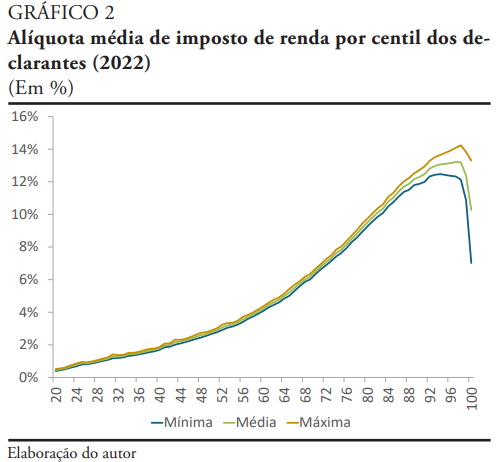
\includegraphics[width=0.6\textwidth]{aliquota.png}
    \caption{Average tax rate by income percentile}
    \label{tab:Figure 1}
\end{figure}

{\Large{\textit{Translation:}}}
\\
\\
Average tax rate by income percentile among reporters (2022).
\\
(As a \%)
\\
\textcolor{blue}{\textbf{---}} Minimum \textcolor{darkgreen}{\textbf{---}} Average \textcolor{orange}{\textbf{---}} Maximum.
\\
Source: IBGE, 2022.
\\
\begin{figure}[H]
    \centering
    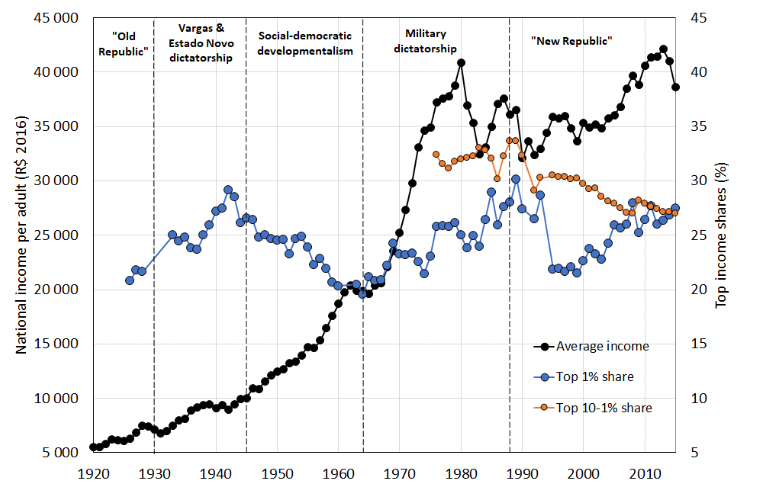
\includegraphics[width=0.6\textwidth]{oneperc.png}
    \caption{Average income over time}
    \label{tab:Figure 2}
\end{figure}

\end{document}